\documentclass[crop,tikz]{standalone}% 'crop' is the default for v1.0, before it was 'preview'
\usetikzlibrary{positioning,shapes.geometric}

\begin{document}

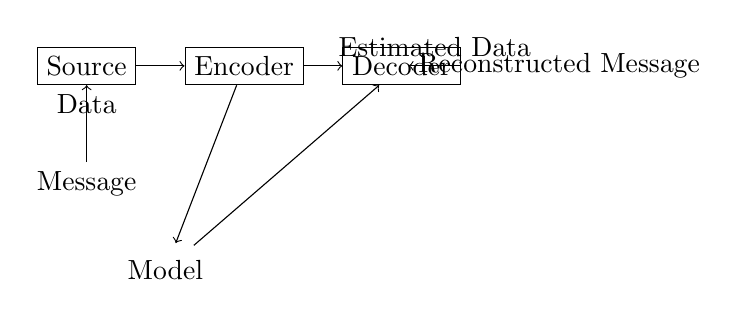
\begin{tikzpicture}[node distance=2cm,auto]
    % Nodes
    \node[draw, rectangle] (source) {Source};
    \node[below of=source, node distance=1.5cm] (message) {Message};
    \node[draw, rectangle, right of=source] (encoder) {Encoder};
    \node[draw, rectangle, right of=encoder] (decoder) {Decoder};
    \node[right of=decoder] (reconstructed) {Reconstructed Message};
    
    % Arrows
    \draw[->] (message) -- node[above] {Data} (source);
    \draw[->] (source) -- (encoder);
    \draw[->] (encoder) -- (decoder);
    \draw[->] (decoder) -- node[above] {Estimated Data} (reconstructed);
    
    \node[ellipse, below=of encoder, xshift=-1cm] (model) {Model};
    \draw[->] (encoder) -- (model);
    \draw[->] (model) -- (decoder);
    
\end{tikzpicture}

\end{document}
